
\section{Background}

Epilepsy ranks among the most common long-term neurological conditions worldwide. The World Health Organization estimates that roughly 50 million people live with epilepsy globally, spanning all age groups, geographies, and socioeconomic backgrounds~\citep{who2019epilepsy, chanu2023automated}. The disorder manifests through recurrent seizures, which are brief episodes of involuntary movement, altered consciousness, or unusual sensations triggered by sudden, synchronized bursts of abnormal electrical activity in the brain. What makes epilepsy especially dangerous is its unpredictability; a seizure can occur while a person is cooking, crossing a road, or sleeping.

The electroencephalogram (EEG) has been the workhorse of epilepsy diagnosis for decades. Thin electrodes placed on the scalp pick up the electrical signals generated by large populations of neurons, tracing them as oscillating waveforms over time. A trained neurologist can distinguish the high-amplitude, chaotic spikes of a seizure from the relatively calm rhythms of healthy brain activity. But this visual inspection is far from straightforward. A routine clinical EEG recording might run for half an hour; continuous monitoring in intensive care can stretch to several days. Scanning through all that data to spot episodes that may last only a few seconds demands considerable time, focus, and expertise~\citep{adeli2003analysis}.

\section{Problem Statement}

The manual review of EEG recordings for seizure detection suffers from several well-documented problems. First, it is extremely labour-intensive. A neurologist must carefully examine hours of waveform data to locate brief seizure events that can easily be missed during a lapse in attention. Second, the process is inherently subjective. Two experienced clinicians may look at the same stretch of EEG and arrive at different conclusions, especially for borderline or ambiguous patterns~\citep{chanu2023automated}. Third, there is a global shortage of trained EEG specialists, particularly in rural clinics and low-resource settings, leading to long waiting times and delayed diagnoses.

These challenges have motivated researchers to explore automated approaches. Over the past decade, a range of machine learning methods have been proposed to assist clinicians by flagging potential seizure events in EEG data. However, many of these systems share one or more of the following weaknesses:

\begin{enumerate}[leftmargin=2cm]
    \item They extract features from only one or two signal analysis domains (typically wavelets alone), overlooking complementary information that other domains could contribute.
    \item They depend on a single classifier, which may not generalize well across different patient populations or recording conditions.
    \item They offer no form of interpretability; the model outputs a decision but provides no explanation for why it arrived at that conclusion. In clinical settings, this opacity erodes trust and limits practical adoption.
\end{enumerate}

\section{Motivation}

Two observations drive this project. The first is that most existing seizure detection systems operate as black boxes. A physician receives a verdict, either ``seizure detected'' or ``normal'', without any insight into the signal characteristics that led to that judgement. In a medical context, where the stakes are high and accountability matters, this is a serious limitation. Clinicians want to see the evidence, not just the conclusion.

The second observation is that the feature engineering in prior works is often narrow. Chanu et al.~\citep{chanu2023automated} showed that discrete wavelet transform (DWT) features paired with an optimized neural network can reach 99.2\% accuracy on the Bonn dataset. Chen et al.~\citep{chen2023epileptic} demonstrated that combining DWT-based entropy features with a Random Forest selector and a CNN classifier can achieve high accuracy across multiple binary classification tasks on the same dataset. Both studies confirmed the usefulness of wavelet-based analysis, but neither explored a broad, multi-domain feature set, and neither integrated any form of post-hoc explainability.

This project builds on those ideas in three specific ways:

\begin{itemize}
    \item It extracts a much larger feature set of 720 features spanning four different analysis domains, namely wavelet, time, frequency, and nonlinear, capturing a wider range of the signal's behaviour.
    \item It replaces single-model classification with an ensemble of eight distinct classifiers combined through soft voting and multi-seed averaging, improving both accuracy and stability.
    \item It integrates SHAP-based explanations into every prediction, so that each output comes with a transparent account of which features contributed to it and by how much.
\end{itemize}

\section{Objectives}

The key objectives of this project are:

\begin{enumerate}[leftmargin=2cm]
    \item To preprocess raw EEG recordings from the Bonn University dataset using a fourth-order Butterworth bandpass filter (0.5--85~Hz) and z-score normalization.
    \item To engineer a comprehensive set of 720 features from each signal, covering discrete wavelet transform coefficients, time-domain statistics, frequency-domain band powers, and nonlinear complexity measures.
    \item To apply a union-based feature selection strategy combining mutual information and ANOVA F-classification scores, retaining only the most discriminative features.
    \item To train a soft-voting ensemble of eight classifiers, namely Random Forest, Extra Trees, Histogram Gradient Boosting, SVM, MLP, Gradient Boosting, AdaBoost, and KNN, and evaluate it through 10-fold stratified cross-validation.
    \item To integrate SHAP (SHapley Additive exPlanations) for model transparency, producing global feature importance rankings, SHAP summary plots, and permutation importance analysis.
    \item To deploy the trained pipeline as a Flask-based REST API backed by a web dashboard where users can upload EEG files, view predictions, and inspect explanations.
\end{enumerate}

\section{Scope of the Project}

This project is scoped to the Bonn University EEG dataset, which contains 500 single-channel recordings distributed across five clinical categories. The classification task is binary: seizure (Set~E) versus non-seizure (Sets~A through~D). The system is designed as a proof-of-concept demonstrating that ensemble learning combined with explainable AI can deliver both high accuracy and clinical transparency. It does not aim to replace the judgement of a neurologist; rather, it is intended to serve as an assistive screening tool that can speed up initial triage.

\section{Project Timeline}

Development was carried out over four months, from January to April 2026, organized into six overlapping phases. Figure~\ref{fig:timeline} presents the schedule.

\begin{figure}[H]
\centering
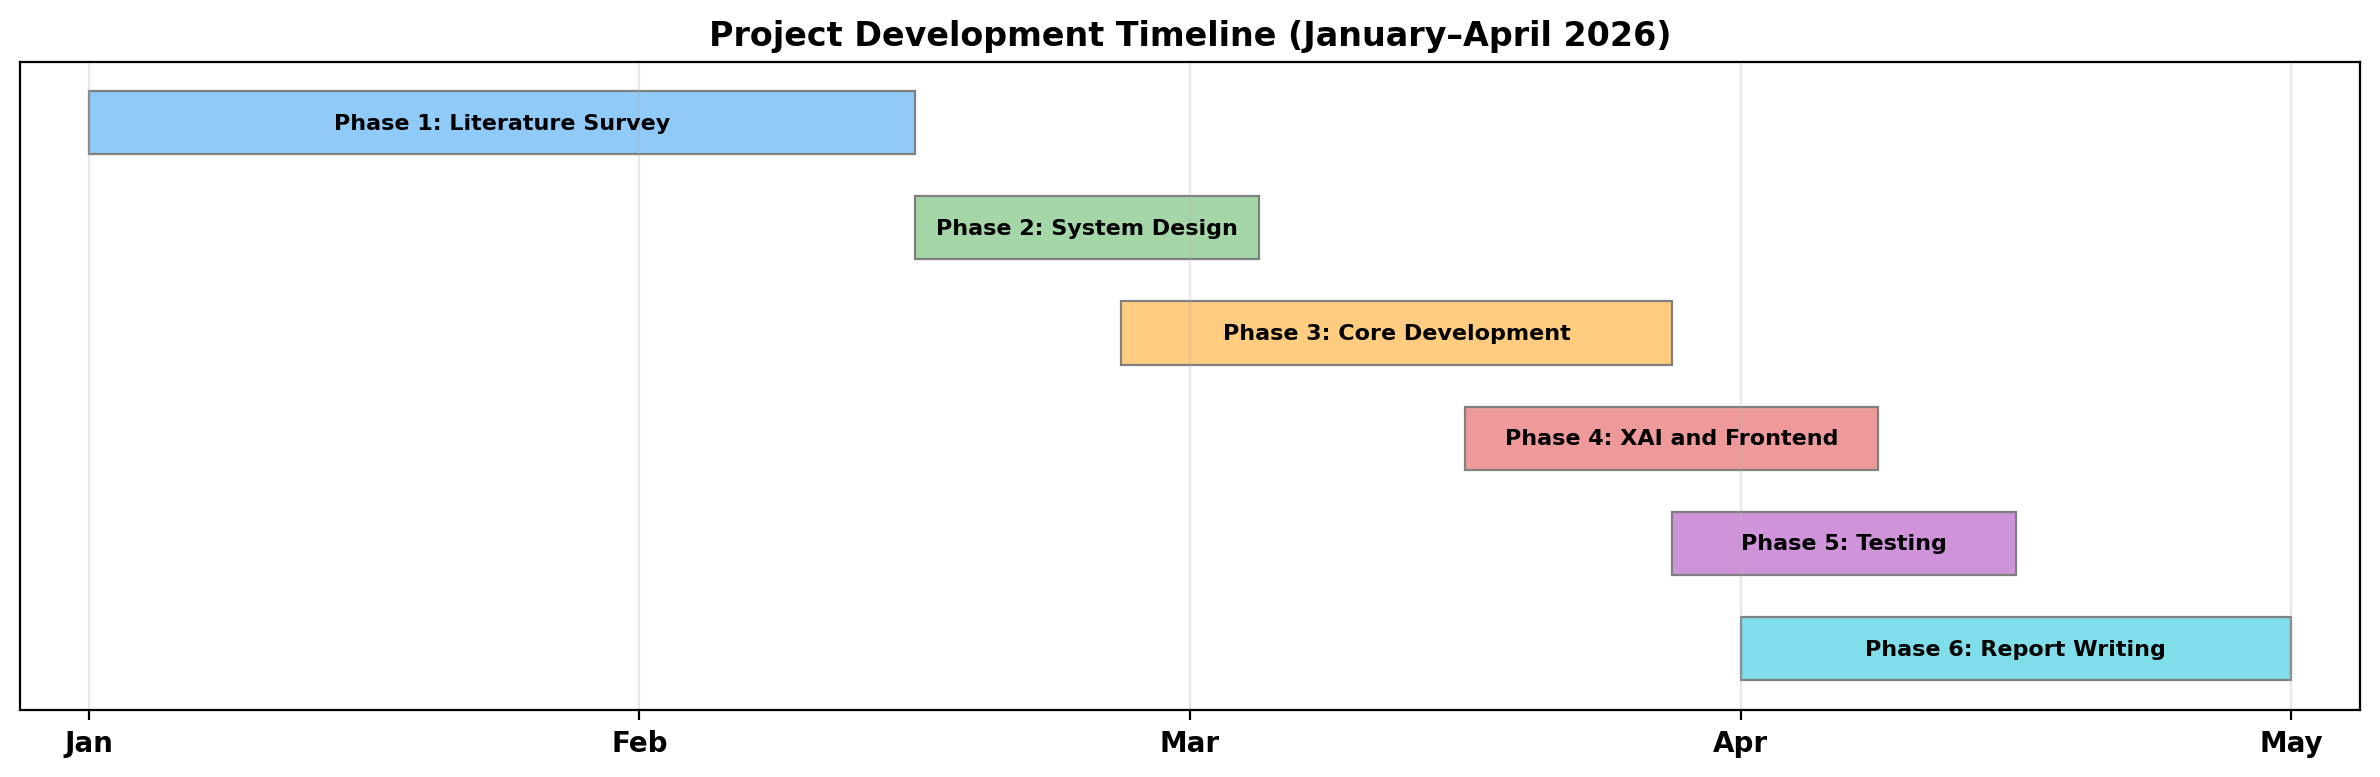
\includegraphics[width=\textwidth]{images/gantt_chart.png}
\caption{Project development timeline (January--April 2026).}
\label{fig:timeline}
\end{figure}

\begin{itemize}
    \item \textbf{Phase~1 (January--mid February):} Studying existing seizure detection methods, reading the base papers by Chanu et al. and Chen et al., understanding the Bonn dataset, and identifying gaps in current approaches.
    
    \item \textbf{Phase~2 (mid February--late February):} Deciding on the modular pipeline architecture, choosing the feature domains and classifiers, and setting up the project directory structure.
    
    \item \textbf{Phase~3 (late February--mid March):} Implementing the data loader, signal preprocessing module, multi-domain feature extraction (720 features), and the eight-classifier ensemble with multi-seed training.
    
    \item \textbf{Phase~4 (mid March--late March):} Adding SHAP-based explainability, building the Flask REST API, and developing the frontend dashboard with EEG visualization.
    
    \item \textbf{Phase~5 (late March):} End-to-end testing, debugging, validating metrics under cross-validation, and ensuring the API and frontend work correctly together.
    
    \item \textbf{Phase~6 (April):} Writing the project report, compiling results, generating figures and tables, and preparing the final submission.
\end{itemize}

\section{Organization of the Report}

The remainder of this report is laid out as follows. Chapter~2 surveys existing literature on automated seizure detection, discussing the strengths and shortcomings of earlier methods. Chapter~3 covers requirements engineering, including feasibility analysis, use case modelling, and the software requirement specification. Chapter~4 describes the system design with architecture diagrams, data flow, and module-level design. Chapter~5 presents the implementation in detail, along with formal algorithms for the core components. Chapter~6 reports the experimental results, classification metrics, and a comparison with related work. Chapter~7 concludes the report with a summary of contributions and directions for future work.
